
%(BEGIN_QUESTION)
% Copyright 2006, Tony R. Kuphaldt, released under the Creative Commons Attribution License (v 1.0)
% This means you may do almost anything with this work of mine, so long as you give me proper credit

En oppfinnsom krets som brukes til å generere et elektrisk spenningssignal fra en differensiell kapasitanssensor er {\it Twin-T diodekretsen}, vist her koblet til en Rosemount-aktig differensiell kapasitans-trykksensor:

$$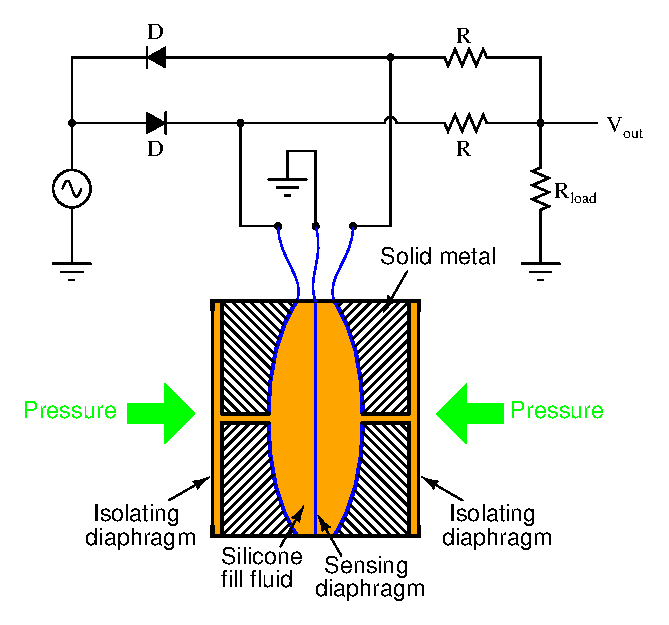
\includegraphics[width=15.5cm]{i00023x01.eps}$$

Den ene kondensatoren lades positivt i forhold til jord, mens den andre lades negativt i forhold til jord, ettersom AC-spenningskilden veksler mellom positiv og negativ.  Mens den ene kondensatoren i trykksensoren lades, utlades den andre gjennom $R_{load}$, og produserer en utgangsspenning ($V_{out}$).

Hvis begge kapasitansene er like, vil utgangsspenningen veksle likt mellom positive og negative verdier, med en DC-gjennomsnittsverdi på null.  Hvis den ene kapasitansen er større enn den andre, vil den lagre ekstra ladning på platene, som forskyver utgangsspenningen til Twin-T-kretsen i retning av dens polaritet.  Dermed blir $V_{out}$ mer positiv når trykket øker på den ene siden av sensoren, og mer negativ når trykket øker på den andre siden av sensoren.

\vskip 10pt

Basert på denne forklaringen av Twin-T-kretsens virkemåte, avgjør hvilken side av den viste differensielle kapasitanssensoren som er "High"-trykksiden, og hvilken som er "Low"-trykksiden.  Forklar resonnementet ditt!

\vfil

\underbar{file i00023}
\eject
%(END_QUESTION)





%(BEGIN_ANSWER)

Dette er et vurdert spørsmål -- ingen svar eller hint gis!

%(END_ANSWER)





%(BEGIN_NOTES)

Husk at "High"-trykkporten på et DP-instrument er den som gjør at instrumentets indikasjon blir mer positiv når trykk påføres.  For at denne Twin-T-kretsen skal gi et mer positivt utgangssignal, må kondensatoren som lagrer den positive ladningen ha større kapasitans enn kondensatoren som lagrer den negative ladningen.

Ut fra diodenes orientering ser vi at venstre halvdel av den differensielle kapasitanscellen er kondensatoren som lagrer den positive ladningen.  For å gjøre dens kapasitans større må den fleksible målemembranen i midten bevege seg nærmere den venstre, faste platen.  Dette betyr at det må være større trykk på høyre side av cellen, som gjør høyre side til "High"-trykksiden.

$$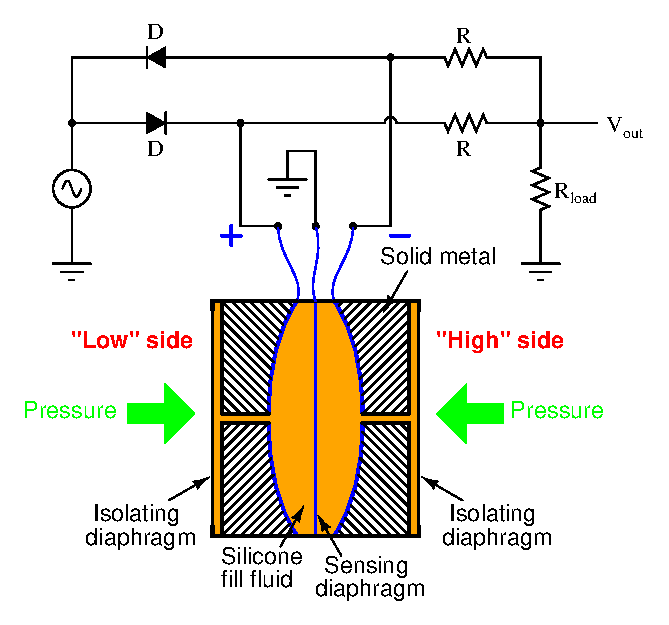
\includegraphics[width=15.5cm]{i00023x02.eps}$$



%INDEX% Measurement, pressure: differential capacitance cell

%(END_NOTES)
